\documentclass{awac02}

% Packages
\usepackage[utf8]{inputenc}
\usepackage{tabularx}
\usepackage{graphicx}
\usepackage{svg}
\usepackage{tikz}
\usepackage{xparse}
\usetikzlibrary{positioning, fit, backgrounds, shapes, arrows.meta}

% State machine

\tikzstyle{base} = [minimum width=3cm, minimum height=1cm, node distance=2em, text centered, draw=black, inner sep=5pt]

\tikzstyle{start} = [base, rectangle, rounded corners, draw=black, fill=red!30]

\tikzstyle{io} = [trapezium, trapezium left angle=70, trapezium right angle=110, 
 minimum height=1cm, text centered, draw=black, fill=blue!30, trapezium stretches=true,
 align=center, inner sep=1em] 

\tikzstyle{state} = [base, rectangle, fill=orange!30]

\tikzstyle{decision} = [base, rectangle, rounded corners=0.8em, fill=green!30]

\tikzstyle{subprocess} = [rectangle, draw = black!50, minimum height = 2em, fill=pink!50]

\tikzstyle{process2} = [rectangle, minimum height=1cm, align=center, draw=black, fill=yellow!30, inner sep=1.8em]

\tikzstyle{process_label} = [external/.style={draw=black!50}, font={\fontsize{13pt}{12}\selectfont}]

\tikzstyle{arrow} = [thick,->,>=stealth]
\tikzstyle{slow_arrow} = [dotted, thick,->,>=stealth]
\tikzstyle{line} = [thick]

\NewDocumentCommand\StateWithBullets{m m m >{\SplitList{;}}m}{%
    \node (#1) [state, text width=6cm, #2, inner sep=5pt] {\large #3\small \begin{itemize}
    \ProcessList{#4}{\insertitem} \end{itemize}};
}
\newcommand\insertitem[1]{\item #1}

\NewDocumentCommand\JustBullets{m m >{\SplitList{;}}m}{%
    \node (#1) [state, text width=3.5cm, #2, inner sep=5pt, rounded corners,
    fill=blue!30] {\vspace{-0.8em}\small\begin{itemize}
    \ProcessList{#3}{\insertitem} \end{itemize}};
}

% Distances
\newcommand{\shortarrowlength}{3.1em}

% Menu
\tikzstyle{menu-base} = [text centered, draw=black, inner sep=0.5em, node
distance=4em, minimum height=3em, minimum width=9em]

\tikzstyle{menu-enterexit} = [menu-base, rectangle, rounded corners, fill=black!10]

\tikzstyle{menu-item} = [menu-base, rectangle, rounded corners, minimum height=3.5em]

\tikzstyle{menu-small-item} = [menu-base, rectangle, rounded corners, minimum
width=4em, minimum height=2em]

\tikzstyle{menu-setting} = [menu-base, rectangle, rounded corners, minimum
width=7em]

\tikzstyle{button-label} = [circle, draw=black, minimum size=1.3em, fill=white, inner
sep=0, line width=0.5pt, font=\footnotesize]

\tikzstyle{menu-single} = [->, >={Latex[length=2mm, width=3mm]}, line width=4pt]
\tikzstyle{menu-double} = [menu-single, <->]

\newcommand{\LRvert}[2]{%
    \draw[menu-single] ([xshift=1em]#1.south) -- node[button-label] {R}
        ([xshift=1em]#2.north);
    \draw[menu-single] ([xshift=-1em]#2.north) -- node[button-label] {L}
        ([xshift=-1em]#1.south);
}

\newcommand{\LRhor}[2]{%
    \draw[menu-single] ([yshift=0.5em]#1.east) -- node[button-label] {R}
        ([yshift=0.5em]#2.west);
    \draw[menu-single] ([yshift=-0.5em]#2.west) -- node[button-label] {L}
        ([yshift=-0.5em]#1.east);
}

\newcommand{\IncrementDecrementNode}[2]{%
    \node (_#2anchor) [#1=\shortarrowlength+1.3em of #2, outer sep=1pt, inner sep=0] {};
    \node (_#2L) [button-label, above left=0.2em of _#2anchor] {L};
    \node (_#2dec) [below left=0.2em of _#2anchor, inner sep=0, circle, minimum size=1.3em] {--};
    \node (_#2R) [button-label, above right=0.2em of _#2anchor] {R};
    \node (_#2inc) [below right=0.2em of _#2anchor, inner sep=0, circle, minimum size=1.3em] {+};
    \node (_#2set) [fit={(_#2L) (_#2R) (_#2dec) (_#2inc)}, draw] {};
}

\newcommand{\SetTimeNode}[3]{%
    \node (#1) [#2, menu-small-item] {#3};
    \IncrementDecrementNode{below}{#1}
    \draw[menu-double] (#1) -- node[button-label] {SP} (_#1set.north);
}



\title{Documentation}

\begin{document}

\maketitle

\section{Overview}

The documentation is meant as a guide for the developer. Additional aid is
found in the source header files where most functions are documented.

\section{Source Files}

In this section an overview of the project files are given.
The files are listed in order of relevance.

\begin{centering}
\vspace{3mm}
\begin{tabularx}{.9\textwidth}{ >\raggedright p{5cm} | X }
    File(s)                  & Description \\ [0.5ex]
    \hline
    \texttt{main.c}                     & The main file. Contains the
                                          state-machinde.\\
    \texttt{constants.h}                & Global constants for defining number
                                          of displays, enabling logging etc. \\
    \texttt{log.h}, \texttt{log.c}      & Logging functions. Everything here
                                          will be unavailable if the LOG
                                          constant is undefined. \\
    \texttt{rtc.h}, \texttt{rtc.c}      & High level functions to set and show
                                          the external RTC clock. \\
    \texttt{display.h}, \texttt{display.c} & Low level functions to interface
                                             with the Qwiic Alphanumeric Display \\
    \texttt{helpers.h}, \texttt{helpers.c} & Simple helper-functions. \\
    \texttt{external\_interrrupts.h}, \texttt{external\_interrupts.S} & 
                    Register and extract the external interrupts (button
                    presses and RTC alarms). \\
    \texttt{time.h}, \texttt{time.S}    & Start and use the hardware times. \\
    \texttt{sleep.h}, \texttt{sleep.S}  & Set the processor sleep state. \\
    \texttt{twi.h}, \texttt{twi.S}      & Interface to the TWI (I2C) hardware.
                                          Read and write to external devices. \\
    \texttt{eeprom.h}, \texttt{eeprom.S} & Read and write to the EEPROM
                                           (non-volatile storage). \\
    \texttt{flash.h}, \texttt{flash.S}  & Read constant data from flash. For
                                          example an ASCII conversion table. \\
    \texttt{io.h}, \texttt{io.S}        & Direct control of pins. \\
    \texttt{usart.h}, \texttt{usart.S}  & Send data through USART. This is used
                                          to implement printf in `log.c` \\
    \texttt{math.S}                     & Low level math for assembly routines.
\end{tabularx}
\end{centering}

\section{Schematic}

In figure \ref{fig:schematic} the schematics is shown. The schematic is found
seperatly in the \texttt{hardware} directory.

\begin{figure}[h]
    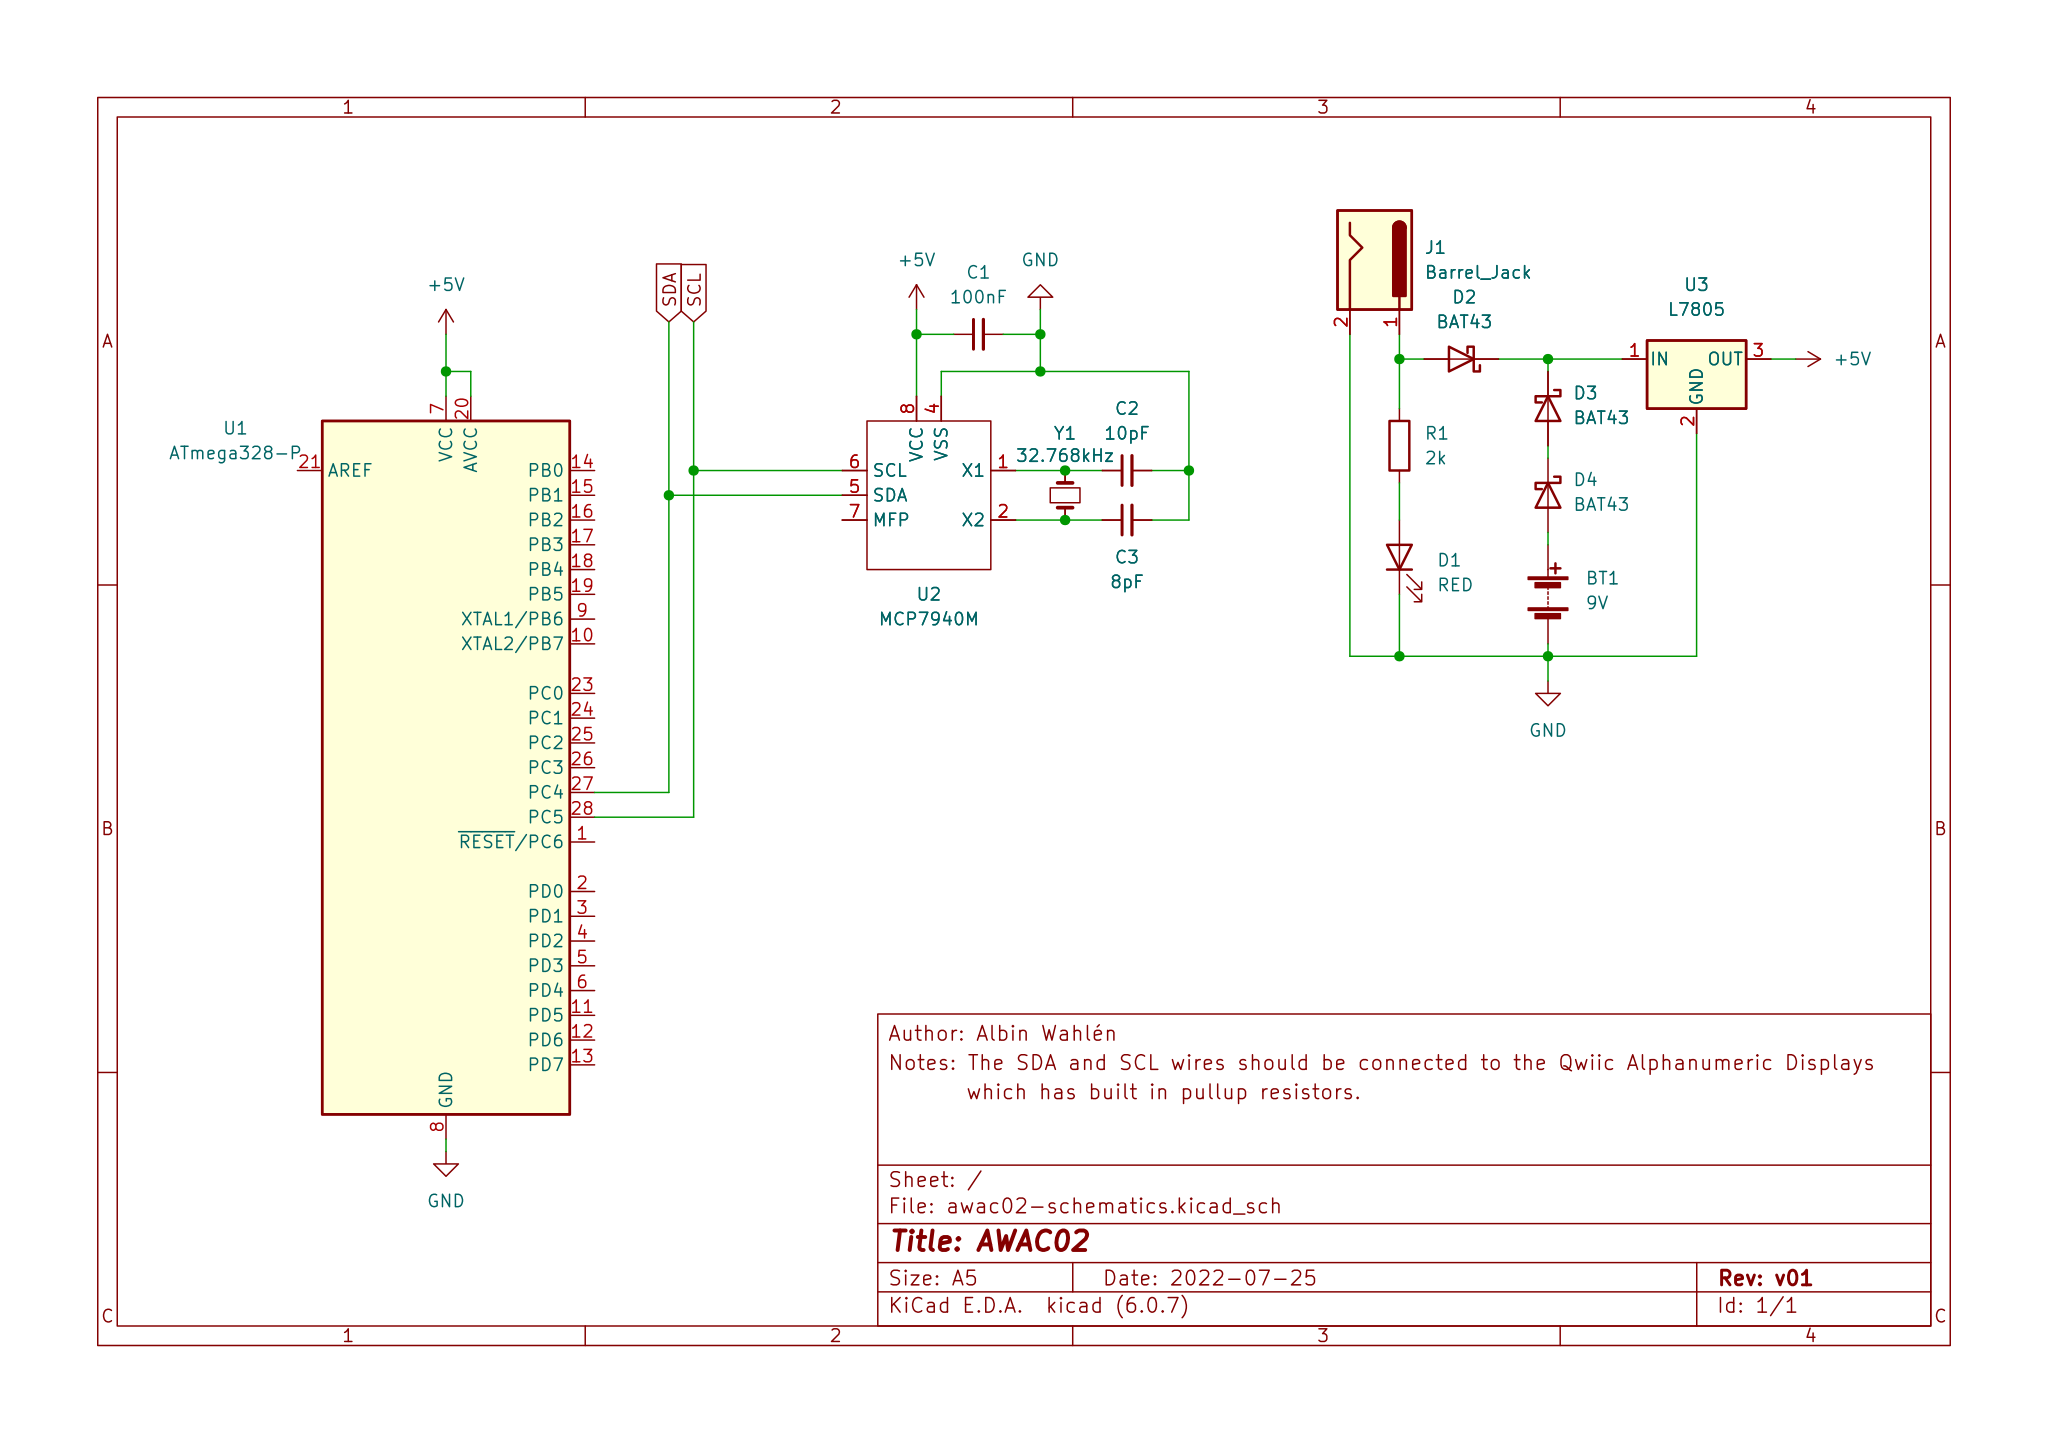
\includegraphics[width=\textwidth]{../hardware/AWAC02-v01}
    \label{fig:schematic}
\end{figure}

\section{State Machine}

The state machine is in \texttt{main.c}. It is implemented using the
\texttt{goto} statement which can lead to hard to understand code. To make
development of the state machine easier all states are documented here and
shown in a flow-chart. The program starts in the \texttt{enter\_clock\_mode}
state.

\vspace{5mm}
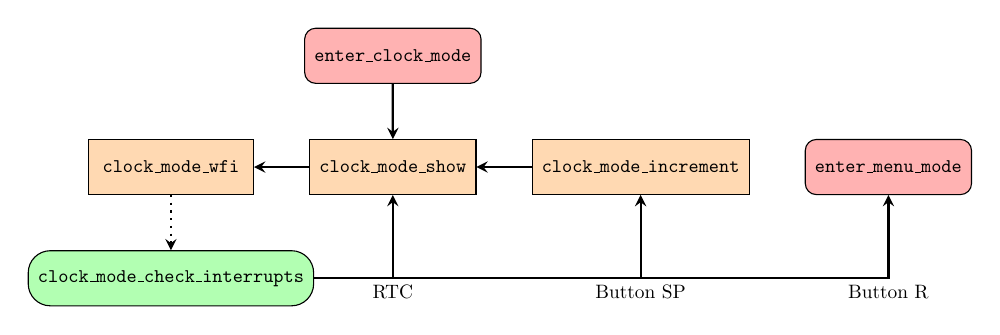
\begin{tikzpicture}[every node/.style={scale=0.7}]

\node (CLOCK_MODE_SHOW) [state] { \texttt{clock\_mode\_show}};
\node (ENTER_CLOCK_MODE) [start, above=of CLOCK_MODE_SHOW] {\texttt{enter\_clock\_mode}};
\node (CLOCK_MODE_INCREMENT) [state, right=of CLOCK_MODE_SHOW] {\texttt{clock\_mode\_increment}};
\node (CLOCK_MODE_WFI) [state, left=of CLOCK_MODE_SHOW] {\texttt{clock\_mode\_wfi}};
\node (CLOCK_MODE_CHECK_INTERRUPTS) [decision, below=of CLOCK_MODE_WFI] {\texttt{clock\_mode\_check\_interrupts}};
\node (ENTER_MENU_MODE) [start, right=of CLOCK_MODE_INCREMENT] {\texttt{enter\_menu\_mode}};

\draw [arrow] (ENTER_CLOCK_MODE) -- (CLOCK_MODE_SHOW);

\draw [arrow] (CLOCK_MODE_CHECK_INTERRUPTS) -| node[anchor=north]{RTC}
    (CLOCK_MODE_SHOW);
\draw [arrow] (CLOCK_MODE_CHECK_INTERRUPTS) -| node[anchor=north]{Button SP} (CLOCK_MODE_INCREMENT);
\draw [arrow] (CLOCK_MODE_CHECK_INTERRUPTS) -| node[anchor=north]{Button R} (ENTER_MENU_MODE);

\draw [arrow] (CLOCK_MODE_SHOW) -- (CLOCK_MODE_WFI);
\draw [arrow] (CLOCK_MODE_INCREMENT) -- (CLOCK_MODE_SHOW);
\draw [slow_arrow] (CLOCK_MODE_WFI) -- (CLOCK_MODE_CHECK_INTERRUPTS);

\end{tikzpicture}


\end{document}
